In this chapter a survey of pervasive healthcare applications is presented. In order to gain a greater understanding of which are the building blocks of a typical \acf{IoT} system, a reference model is also presented.

% Aqui é necessário algum contexto ao leitor. Uma vez que vais entregar um estado da arte, é dificil desacoplares isto completamente do teu trabalho.
% Seria importante uma frase introdutória do estilo:
% "Being central to the work described in this dissertation/report/document, in this chapter..."

\todo[inline]{To-do: Redo introductory paragraph (see coments in latex).}

\section{Internet of Things}

\subsection{Fundamentals of \acs{IoT}}

% Por ser tão central ao trabalho, colocar a definição dentro de uma caixa para ficar mais realçada pode fazer sentido. Avalia isso.

\acl{IoT} (or \acs{IoT}) is an emerging communication paradigm, often hailed as the driver of the Fourth Industrial Revolution \cite{Aceto2020}. \bigskip

\todo[inline]{To-do: Highlight definition using a box (see coments in latex).}

The definition of this concept has evolved over time with the development of other technologies such as data analytics, embedded systems, sensors, etc. Fundamentally, it describes a strategy supported on the development of networks of smart devices that exchange and process information through Machine-to-Machine (M2M) communications, usually based on the \acf{IP} \cite{Baker2017}. This technology enables ubiquitous systems to gather remarkable amounts of information regarding the surrounding environment, which can later be turned into insight through the usage of data fusion and data analytics tools, like Machine Learning. \bigskip

In the specific context of healthcare, this technology can provide many benefits as it enables remote and continuous health monitoring \cite{Doukas2012, Wu2020, Fan2014}. It allows non-critical patients to be monitored from the comfort of their own houses, rather than in hospitals or clinics, reducing the strain on scarce hospital resources such as health professionals or beds. This is particularly beneficial to those who live in rural areas, with limited access to healthcare services. It enables elderly people and those with chronic diseases to have greater control over their own health, thus allowing them to live more independently. Moreover, with the automatization of medical procedures, these systems can make healthcare infrastructures more efficient and therefore lower the costs of healthcare \cite{Catarinucci2015, Adame2018}. Particularly, in the realm of clinical research, by analyzing the data collected by these ubiquitous systems, it may be possible to find new relationships between certain pathologies and different physiological signals, such as variations in body temperature or heart rate \cite{Choi2016}. These correlations, commonly referred to as biomarkers, can be used by these systems to assist clinical decisions, enabling novel predictive, prognostic, and diagnostic processes in healthcare.

\section{A Reference Model for Pervasive Healthcare Applications}

Reference models provide an abstract framework for designing systems and a set of commonly recommended practices for the application domain. It serves as a starting point in the design process, enabling the comprehension of complex systems by breaking them down into simple and distinct functional layers, while also defining some common terminology used in its domain. \bigskip

In 2014, the \acs{IoT} World Forum (IoTWF) architectural committee published an \acs{IoT} architectural reference model, composed by seven layers as shown in Figure \ref{fig:iotwf-referencemodel}. This model \cite{Cisco2014} provides a simple and clean functional view into the different components of an \acs{IoT} system, without narrowing the scope or locality of its components. However, from a hardware perspective, in this work we will focus on the most common approach taken by researchers, using 3 distinct components: 

\begin{itemize}
    \item \textbf{Endpoint} or \textbf{edge} nodes (corresponding to Layer 1), which interact with the physical world, capturing data.
    \item \textbf{Gateway} devices (Layer 3), which connect to one or multiple \textbf{edge} nodes, filtering and aggregating the data generated by these and communicating it to a central server; 
    \item \textbf{Central} server (Layers 4-6), which is responsible for collecting, storing and analyzing the captured data in order to provide users with valuable insight;
\end{itemize}

While this model can be used to generically develop \acs{IoT} systems for any industry (\textit{e.g.} from agriculture to smart cities), in the context of the dissertation we will focus on pervasive healthcare applications. \bigskip

\todo[inline]{To-do: Make new image based on this one. (!!)}

\begin{figure}[H]
    \centering
    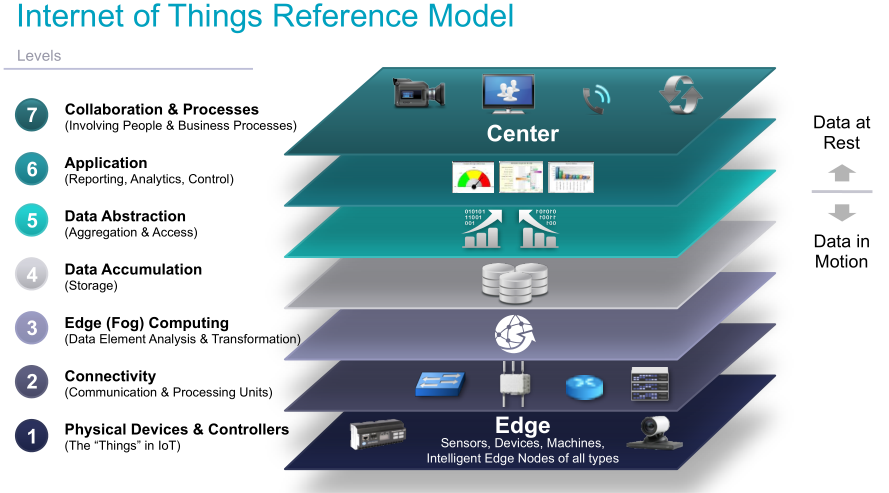
\includegraphics[width=0.85\linewidth]{images/iotwf-referencemodel.png}
    \caption[IoT reference model published by IoTWF.]{IoT reference model published by IoTWF. Source: \cite{Cisco2014}.}
    \label{fig:iotwf-referencemodel}
\end{figure}

\subsection{Layer 1: Physical Devices and Controllers}
\label{sec:iot-model-layer1}

The first layer of the model \cite{Cisco2014} corresponds to the physical devices and controller layer. This layer houses the ``things in the \acl{IoT}: the endpoint devices composed of sensors and actuators that perceive and interact with the physical world. Through those interactions, the devices generate data, which is then sent across the network for analysis and storage. \bigskip

Wearable, wireless, and non-intrusive devices are viewed as one of the key components of \acs{IoT}-based healthcare systems \cite{Baker2017}. In recent years there has been remarkable progress on the development of wearable devices, driven by recent technological breakthroughs in the miniaturization of sensors and microfabrication processes \cite{Adame2018, Catarinucci2015}. These devices allow patients to be monitored while retaining their mobility, increasing the comfort of these users. The drawback of this approach lies on the restrictions imposed on the devices. Due to the nature of this technology, most of these units require a portable energy source, which implies reduced memory, computation, and connectivity capabilities in order to minimize energy consumption and maximize their lifetime. Shorter lifetimes translate into higher maintenance costs, as these devices need to be replaced more often. \bigskip

Another point to consider is the data requirements of the system, namely how much data is generated and which type of data is transmitted by each device. Some applications can include a single temperature sensor or heart rate sensor, while more complex systems can include pulse oximetry, electrocardiogram (\acs{ECG}), respiration rate sensors, etc. \cite{Wu2020}. From the literature \cite{Wu2020, Wu2019, Adame2018, MinhDang2019}, the sensors used in these devices can be classified into three distinct categories based on the signals that can be extracted from them, as shown in Table \ref{tab:layer1-sensors}:

\begin{itemize}
    \item \textbf{Physiological Sensors}: used for evaluating the patients health condition.
    \item \textbf{Activity / Motion sensors}: used for detecting fall events, determining the patients location and the travelled distance, estimating the patients body posture, etc.
    \item \textbf{Environmental Sensors}: used for assessing environment conditions and possible hazards, \textit{e.g.} gas leaks in a patients home or an industrial workplace \cite{Wu2019}.
\end{itemize}

\renewcommand{\arraystretch}{2}
\begin{table}[H]
    \centering
    \begin{tabular}{l|l}
        \textbf{Sensor Categories} & \textbf{Examples} \\ 
        \hline
        Vital Signs Monitoring & \makecell{Blood Pressure, \acs{ECG}, PPG, Body Temperature, \\ Respiratory Rate, Galvanic Skin Response, \\ Pulse Oximetry, Glucose Level Sensors} \\
        Activity Monitoring & Accelerometer, Gyroscope, Magnetometer\\
        Environmental Monitoring & Air Temperature, Barometer, Humidity, Gas Sensors \\
    \end{tabular}
    \caption[Type of sensors commonly used in pervasive healthcare applications.]{Type of sensors commonly used in pervasive healthcare applications. Adapted from \cite{MinhDang2019}.}
    \label{tab:layer1-sensors} 
\end{table}
\renewcommand{\arraystretch}{1}

\subsection{Layer 2: Connectivity}
\label{sec:iot-model-layer2}

The second layer of the model focuses on connectivity, on linking the different components of our system, ensuring reliable and timely data transmissions. This includes all communications within the system, which can be divided into two categories: communications within the local network (\textit{e.g.} between edge nodes and the gateway devices), and communications between the edge of the local network (\textit{e.g.} gateway devices) and the central server. \bigskip

\subsubsection{Communication Protocols}

Technology is designed with particular use cases in mind. They catalyze their development so each technology has its own advantages and disadvantages. For instance, short range wireless protocols are limited by transmission range, but long range protocols have a higher energy consumption, which may be unviable for networks with very constrained devices. Each protocol defines their own frame formats and communicates within certain frequency bands, some of which may require licenses. Using licensed frequency bands can provide a better performance as it ensures greater reliability since the network operator grants you exclusivity of frequency spectrum within a certain area. \bigskip

From the literature, a set of key requirements that drive the decision of the communication protocols can be identified \cite{Baker2017, Catarinucci2015, Adame2018}:

\begin{itemize}
    \item \textbf{Energy consumption}: For networks composed of energy constrained devices, the communication protocol should be lightweight and energy efficient in order to maximize the devices lifetime. 
    \item \textbf{Latency}: Certain applications deal with time critical events, for example the detection of health emergencies \cite{Catarinucci2015}. In these cases, any delays in the communications can cause great detriment to the patients well-being, making it crucial to minimize them.
    \item \textbf{Reliability}: Depending on the critical nature of the data that is being communicated, the network stack may need to implement processes such as error-detection, retransmission or handshakes in the communications to ensure more robust transmissions, \textit{e.g.} as implemented in TCP/IP based protocols. Generally, these features come at the cost of greater latency. Therefore, when choosing the communication protocol, a balance must be found between reliability and latency.
    \item \textbf{Security}: Security is one of the most important requirements of any system, but this is especially true for healthcare applications. Due to the sensitive nature of the information, it is crucial to secure it from malicious actors. Communication protocols must implement security mechanisms, such as encryption or data integrity verifications, that ensure the transmissions are not compromised in transit, thus denying third parties the ability to snoop or tamper the transmissions. This issue is studied in depth in \cite{Gope2016}.
    \item \textbf{Interoperability}: To ensure the interoperability of intrinsically different modules of the system it is imperative to choose protocols that are widely accepted and supported in the application domain. This also contributes to the longevity and maintenance of the system, as these will most likely remain supported for longer time periods. 
    \item \textbf{Range}: The communication protocol must ensure the devices can communicate within the required transmission range.
    \item \textbf{Scalability}: These systems contain an enormous amount of devices, which must be uniquely identified. The communication protocol must ensure that every device in the network is addressable, and that performance is not severely impacted by the addition of new devices.
    \item \textbf{Throughput}: The communication protocol should ensure there is enough bandwidth to handle all communications within the designated transmission range. Even within similar technologies, this can vary wildly with the range, as seen in Figure \ref{fig:communication-protocols-throughput}.  

\end{itemize}

\begin{figure}[H] 
    \centering
    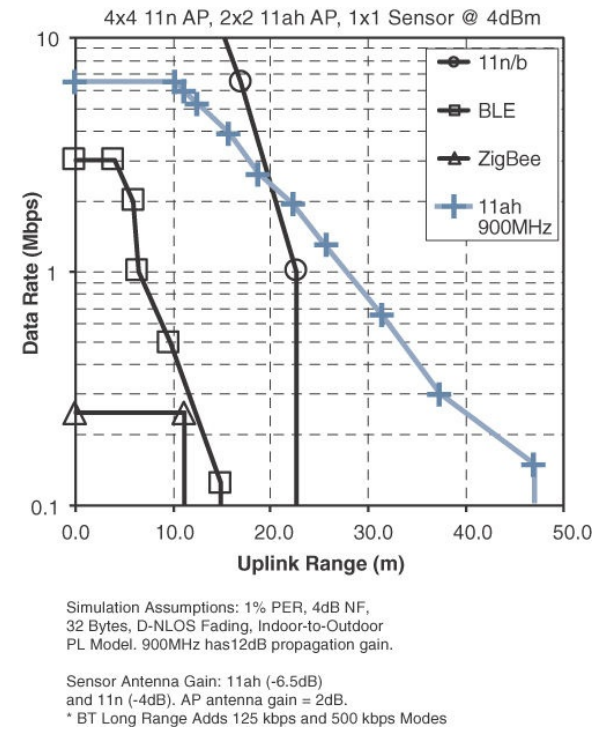
\includegraphics[width=0.55\linewidth]{images/communication-protocols-throughput.png}
    \caption{Throughput versus Transmission range for four communications protocols (quais?) with similar ranges. Source: \cite{10.5555/3161403}}
    \label{fig:communication-protocols-throughput}
\end{figure}

% IEEE 802.15.4?
Regarding communications within the local network, these generally have short transmission ranges \cite{Baker2017}. Wearable devices can be often arranged in networks, aptly designated ``Wireless Body Area Network''. The most widely adopted protocol is \acf{BLE}, a low-energy version of the classic Bluetooth protocol \cite{Doukas2012, Wu2019, Wu2020}. ZigBee and \acf{RFID} are also used in many systems in this domain, particularly in more asset tracking oriented applications \cite{Fuhrer2006, Catarinucci2015, Adame2018}. Despite the absence of a universal specification for \acs{RFID}, the most widely used standard is the EPCglobal Gen2 RFID \cite{EPCglobal2006}, which is the standard considered in this work. For the sake of simplicity, we use \acs{EPC/RFID} to designate it. \bigskip

Out of the abovementioned technologies, \acs{BLE} offers greater throughput, better security, and nearly the lowest energy consumption \cite{dementyev2013power}. Table \ref{tab:comparsion-shortrangeprotocols} shows a comparison between the different protocols.

\renewcommand{\arraystretch}{1.5}
 \begin{table}[H]
     \centering
     \begin{tabular}{r|l|l|l}
         & \textbf{\acl{BLE}} & \textbf{EPC/\acs{RFID}}& \textbf{ZigBee}  \\ \hline
         \textbf{Band of operation} & 2.4 GHz & LF, HF, UHF, EHF & 2.4 GHz \\
         \textbf{Communication} & Bidirectional & \makecell{Unidirectional \\ (Bidirectional for\\ Active tags)} & Bidirectional \\
         \textbf{Topology} & \makecell{ Point-to-Point, Piconet, \\ Broadcast, Mesh } & Point-to-Point & Mesh \\
         \textbf{Range} & <100m & \makecell{<10m, (100m for\\ Active tags)} & 20m \\
         \textbf{Data rate} & 1Mb/s (up to 2Mb/s) & 40kb/s & 250kb/s \\
         \textbf{\acs{IP} Stack} & \xmark & \xmark & \cmark \\
         \textbf{Security Features} & \makecell{AES-128, Secure pairing \\ prior to key exchange} & \xmark & \makecell{AES-128 (Optional),\\ Network key shared \\across network, \\ Optional link key to \\ secure application layer \\ communications}\\
     \end{tabular}
     \caption[Comparison between the more common communication protocols used within short range]{Comparison between the more common communication protocols used within short range. Adapted from \cite{Baker2017}.}
     \label{tab:comparsion-shortrangeprotocols}
 \end{table} 
\renewcommand{\arraystretch}{1}

Regarding communications between the gateway devices and the central server, most researchers try to make use of existing infrastructure in order to facilitate the deployment of new systems. This means, that the communications between the gateway devices and the central server are often done through generic IP-based protocols such as Wi-Fi and Ethernet \cite{Adame2018, Fuhrer2006, Wu2020, Catarinucci2015}. \bigskip

\subsubsection{Application Protocols}
\todo[inline]{To-do: Review this section later.}

So far we have discussed the underlying networking technologies that link the devices in our system. But according to the OSI Model, many of these technologies do not define the application layer: how the devices communicate with each other, how the data is formatted, if there is a hierarchy within the network, etc. When considering networks composed of constrained devices, generic web-based protocols such as Hypertext Transfer Protocol (HTTP) may not be adequate for \acs{IoT} applications, which prompts the development of novel lightweight messaging protocols suited for these systems. The most used application layer protocols in \acs{IoT} systems are \acf{MQTT} and \acf{CoAP}. Table \ref{tab:comparsion-applicationprotocols} overviews these widely used protocols. \bigskip

\renewcommand{\arraystretch}{1.5}
\begin{table}[H]
    \centering
    \begin{tabular}{r|l|l}
        %\textbf{Features} 
        & \textbf{\acs{MQTT}}& \textbf{\acs{CoAP}}  \\ \hline
        \textbf{Transport protocol} & TCP/IP & UDP/IP \\
        \textbf{Messaging pattern} & P-S (asynchronous) & R-R (synchronous) \\
        \textbf{Communication model} & Many-to-many & One-to-one \\
        \textbf{Security} & SSL/TLS (Optional) & DTLS \\
        \textbf{Strengths} & \makecell{TCP and Quality of Service (QoS),\\ robust \\communications, easier to implement } & \makecell{Better for lossy networks,\\ lower latency} \\
        \textbf{Weaknesses} & \makecell{Higher overhead and energy\\ consumption than \acs{CoAP}} & \makecell{Not as reliable and \\less supported than MQTT} \\
    \end{tabular}
    \caption[Comparison between \acs{CoAP} and \acs{MQTT} protocols.]{Comparison between \acs{CoAP} and \acs{MQTT} protocols. Adapted from \cite{10.5555/3161403}.}
    \label{tab:comparsion-applicationprotocols}
\end{table} 
\renewcommand{\arraystretch}{1}

In \cite{Rubi2019}, the authors compare these two protocols in greater length, along with the more commonly used web-based protocol Hypertext Transfer Protocol (HTTP). They analyze the latency in the communications (from the edge devices to remote servers) and the RAM usage in the devices for each protocol and for different data sources (respiration rate, oxygen saturation and heart rate signals) and found that \acs{CoAP} presented the best overall performance. Nonetheless, all protocols had very low latencies (less than 1.5s) and low memory usage. \bigskip

The authors indicate that \acs{MQTT} might be more suitable when considering a certain messaging pattern — the ``Publish/Subscribe (P-S) model. In this model, the devices that send messages, called ``publishers'', communicate them to an intermediary message broker, through a ``message topic (also called logical channels). The devices that wish to receive messages, called ``subscribers'', can subscribe to these topics by requesting it to the message broker. Whenever a publisher sends a message, the broker broadcasts it to all devices that have subscribed to the selected topic. \bigskip

\acs{CoAP} uses a different messaging pattern, called ``Request-Response''. In this paradigm, a device sends a request to receive certain data and the second responds to this request. % observe that the former model is event-driven while the latter is query-based \cite{Rubi2019}. % Due to the nature of how the data is generated in these types of pervasive applications, an event-driven protocol like \acs{MQTT} might be more adequate.

\subsection{Layer 3: Edge (Fog) Computing}
\label{sec:iot-model-layer3}

\acs{IoT} systems may have hundreds or even thousands of sensors generating data multiple times per second, 24 hours per day, which may require an unsustainable amount of network and computing resources. Moreover, certain applications are time critical, where delays in communication can be very detrimental. To minimize these effects, it is crucial to initiate data processing as close to the edge of the network as possible. This paradigm is usually referred to as edge computing, when the data processing occurs at the endpoint devices, or fog computing, when it happens at the edge of local network, \textit{e.g.} in gateway devices. \bigskip

The third layer of the model defines how the system prepares the data for storage and higher level processing for the next layers. However, the endpoint or gateway devices often have limited computing capabilities, so the data processing is generally focused on preprocessing the data in real-time and handling more time critical events. More demanding and thorough data analysis is usually left to the central server. \bigskip

The different processes applied at this stage can be summarized into four distinct categories:

\begin{itemize}
    \item \textbf{Filtering}: Assessing if the data should be processed at a higher level. 
    \item \textbf{Formatting}: Reformatting data to ensure consistent formats for higher-level processing.
    \item \textbf{Cleaning}: Reducing data to minimize the impact of data on the network and higher level processing systems.
    \item \textbf{Evaluation}: Determining whether data represents a threshold or alert. This is especially relevant for applications that deal with time critical events as seen in the previous section.
\end{itemize}

% \todo[inline]{To-do: Add 2 examples of edge computing processes discussed in the systems?} 

\subsection{Layer 4: Data Accumulation}
\label{sec:iot-model-layer4}

The data that is generated by the edge devices is propagated through the system, and eventually reaches the central server. Up to this point, model is event driven. However, most applications cannot make use of the data at the rate it is generated \cite{10.5555/3161403}. In the Data Accumulation layer, we need to define how the system captures the data and stores it, so it becomes usable for applications when needed, thus transiting from event to query-based processing. \bigskip

As the devices continuously generate data, the system will require more and more resources in order to process and store all of this information, raising some concerns regarding how the data can be managed. In \cite{Doukas2012}, the authors propose the usage of cloud platforms as a solution to these problems. This is made possible due to the elasticity in allocating, swiftly and inexpensively, computing and storage resources on-demand, adjusting itself to the needs of each application. Three distinct types of cloud services can be found: %, Figure \ref{fig:differences-between-cloud-services}:

\begin{itemize}
    \item \textbf{Infrastructure as Service (IaaS)}: Provides control over the remote machine (composed of virtual or dedicated hardware), operative system and middleware. This approach gives system designers the highest level of flexibility over the infrastructure, but requires more maintenance.
    \item \textbf{Platform as a Service (PaaS)}: Provides a simple framework for developing applications, where the service provider manages the underlying infrastructure issues such as software updates and hardware maintenance. 
    \item \textbf{Software as a Service (SaaS)}: Provides the finished applications to be used by the end users, in this case health workers, that enable them to work. A simple example is a web-based email service, such as Gmail or Microsoft Outlook. 
\end{itemize}

\begin{figure}[H]
    \centering
    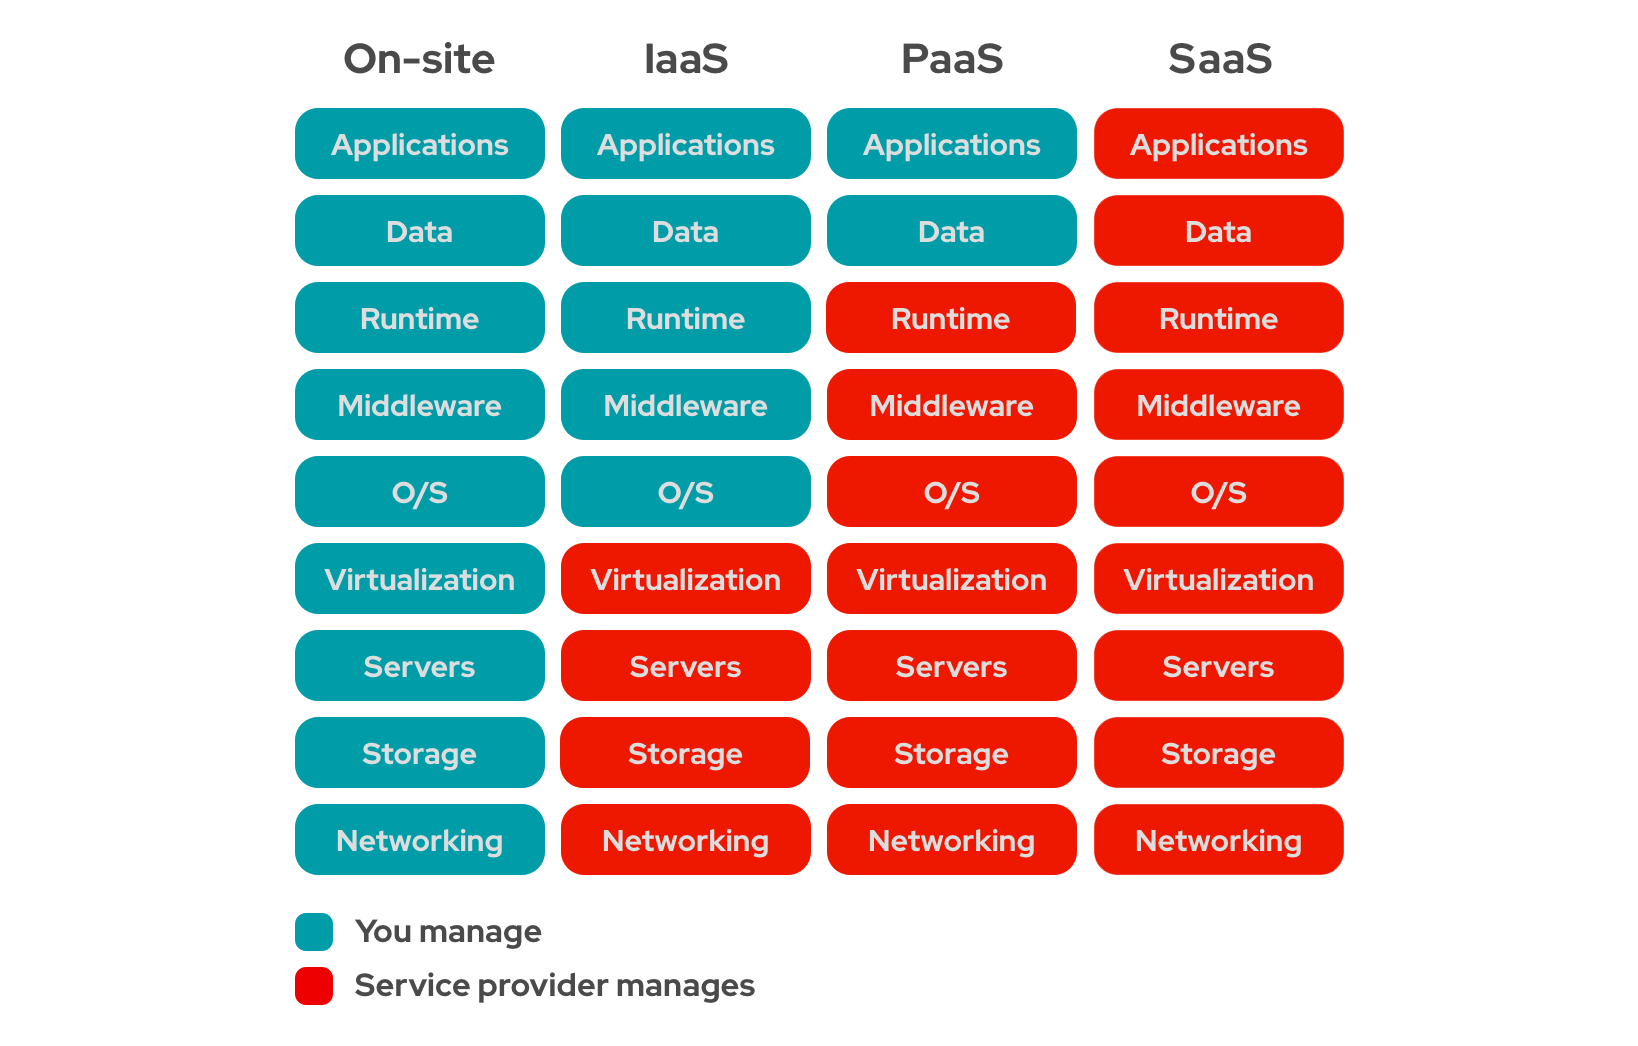
\includegraphics[width=\linewidth]{images/cloud-services.png}
    \caption[Differences between the cloud offerings and on-premise solutions.]{ Differences between the cloud offerings and on-premise solutions. Source: \cite{RedHat2021}}
    \label{fig:differences-between-cloud-services}
\end{figure}

% \todo[inline]{To-do: Should homomorphic encryption methods be discussed? Discuss what is Hadoop? What are the 5 Vs of Big Data?}

Nonetheless, security and privacy remain as key concerns for the implementation of cloud-based solutions. The information must remain accessible to authorized parties such as healthcare providers, but the patients health data has to be kept private. To solve this, there are two commonly adopted features in the literature: access control policies and data encryption \cite{Baker2017}. Access control policies define who can access the data, by authenticating them (validating the identity of the user) and by authorizing them (ensuring that the user has permissions to perform a given operation). Data encryption ensures that, even if the data is leaked, it is still unreadable to third parties, and therefore sensitive information remains secure and private. \bigskip

Regarding storage solutions, most research works use traditional relational databases (SQL) as the means of storing data \cite{Fuhrer2006, Wu2020, Catarinucci2015, Adame2018}. However, as the data is very heterogenous and unstructured, the authors of \cite{Subahi2019} propose using non-relational databases (NoSQL) which can offer much greater flexibility as the schema in these databases is dynamic. Moreover, NoSQL type data stores outperform SQL databases as the data increases in volume \cite{Xu2014}. Table \ref{tab:comparsion-databasetech} illustrates the differences between these two technologies. 

\renewcommand{\arraystretch}{2}
\begin{table}[H]
    \centering
    \begin{tabular}{r|l|l}
        %\textbf{Features} 
        & \textbf{SQL}& \textbf{NoSQL}  \\ \hline
        \textbf{Type of database} & Relational & Non-relational \\
        \textbf{Database model} & Table-based database & \makecell{Document-based databases, Key-value stores, \\ graph stores, wide column stores} \\
        \textbf{Data type} & Appropriate for structured data & Appropriate for unstructured or semi-structured data \\
        \textbf{Schema} & Strict schema & Dynamic schema \\
        \textbf{Query} & \makecell{Uses Standard Query \\Language (SQL), appropriate for \\ complex query operations} & \makecell{Uses Unstructured Query \\ Languages (\textit{e.g.} UnQL), does not support \\ complex query operations}  \\ 
        \textbf{Scalability} & Vertical & Horizontal \\
        \textbf{Performance} & Lower than NoSQL & Optimized for large datasets \\
    \end{tabular}
    \caption{Comparison between SQL and NoSQL technologies.}
    \label{tab:comparsion-databasetech}
\end{table} 
\renewcommand{\arraystretch}{1}

\subsection{Layer 5: Data Abstraction}
\label{sec:iot-model-layer5}

\todo[inline]{To-do: Complete section (develop FHIR section).} 

In the previous layer, we have defined how the system captures the information. In some cases, the collection of data may require the development of multiple concurrent storage solutions, each using different technologies, resulting in a very complex environment. The purpose of this layer is to develop services that simplify how the applications access the data, to reconcile the different data stores and ensure the information is complete and consistent \cite{Cisco2014}. Applications can then interact with these databases through interfaces exposed by these services, designated \acl{API}s (\acs{API}s). \bigskip 

An \acs{API} is a computing interface that defines a set of rules that ``explain how computers and applications communicate with one another, acting as an intermediary between these different components \cite{IBMAPI}. It defines what operations can be performed, how to request them, which are the accepted data types, etc. In this case, it decouples applications from the storage solutions, by encapsulating their functionality behind the interface. This ensures the modularity of the system as the applications become independent of whichever technologies are used in the data stores. \bigskip

Understanding what and how information is shared within the healthcare domain is fundamental. As patients continuously move around the healthcare ecosystem, their health information must be available, discoverable and understandable to different entities (hospitals, laboratories, pharmacies, etc.). This prompts the digitization of medical files and the development of standards for exchanging these records instantly and securely to authorized parties \cite{HL72019}, which are called \acl{EHR}s (\acs{EHR}s). \acs{EHR}s are the digital equivalent of a patients paper-chart, they contain the patients full medical history: previous diagnoses, treatment plans, test results, known allergies, among other details. \bigskip

% Comparison between OpenEHR and FHIR?
One of the most prominent standards for exchanging \acs{EHR}s is \acf{FHIR}. \acs{FHIR} is a standard developed by Health Level Seven International (HL7), which is a non-profit organization involved in the development of international healthcare informatics for over 20 years. \acs{FHIR} builds upon previous data format standards like HL7 v2 and HL7 v3, and is becoming widely adopted within the healthcare industry \cite{Peng2019}. 

% \todo[inline]{To-do: If time allows it, add 2 examples of articles where APIs implemented.} 

\subsection{Layer 6: Application}
\label{sec:iot-model-layer6}

\todo[inline]{To-do: Complete section!}

The sixth layer corresponds to the application layer, where the system ingests the captured data, analyzes it and delivers the value to the end users. Users can then interact with the system through Graphical User Interfaces (UI), which provide different functionalities depending on the application. Some may show simple reports regarding the collected data \cite{Doukas2012, Wu2020}, and others may allow users to monitor and have greater control over the different components of the system. \bigskip

In the healthcare domain, \acs{IoT} applications generally focus on delivering clinical decision support \cite{Gruendner2019,Wagholikar2017,Fan2014, BrainAnswer} and asset tracking \cite{Adame2018, Fuhrer2006, Catarinucci2015} features. Clinical decision support is one of the main drivers for usage of artificial intelligence in medicine\cite{Choi2016}. (...) 

\subsection{Layer 7: Collaboration and Processes}
\label{sec:iot-model-layer7}

% Não removia, uma secção curta e concisa está OK porque não é tão relevante para o trabalho como as outras.
% Podes mencionar, de forma conceptual apenas (não estou a ver nesta fase como operacionalizar no projecto ainda, nem vala a pena especular) o seguinte:
% "Analyze opportunities to improve the efficiency and effectiveness of the processes."
% "Identification of the goals, deliverables, activities, patterns of collaboration, techniques, actions, and % technologies associated with each process."
% Ver:
% https://ieeexplore.ieee.org/document/6148656


The information that is created by the \acs{IoT} yields little value unless it prompts action, which requires people and processes (seventh layer). The objective is not the application — it is to empower people to work better and more efficiently. The sixth layer (Applications) provides business people the right insight, at the right time, so they can make the right decision. To do this people must be able to communicate and collaborate, which often requires multiple steps and transcends multiple applications \cite{Cisco2014}. However, this component of the system is beyond the scope of this work.

\section{Survey on \acs{IoT} Applications for Healthcare}
\label{sec:sim-approaches}

\todo[inline]{To-do: Complete section! 
- Add introductory paragraph! 
Perform a critical analysis of all related work.
You should make clear and focus on what is your contributions, and state clearly what is *not* your contributions (i.e. out of the scope of this work).
Falta um parágrafo introdutório.
O que se vai fazer nesta sub.secção? pq?
}
% \todo[inline]{To-do: Complete section!  Add introductory paragraph!  Perform a critical analysis of all related work. You should make clear and focus on what is your contributions, and state clearly what is *not* your contributions (i.e. out of the scope of this work). Falta um parágrafo introdutório. O que se vai fazer nesta sub.secção? pq }

% This chapter presents a survey of patrolling, surveillance, navigation and exploration strategies already implemented in the literature. In the last decades, related algorithms for multiple robot teams have piqued the interest of the robotics community, becoming a remarkable growing area. One of the main reasons contributing to this fact is the variety of approaches that these algorithms can comprise. Many authors contributed with studies that involve many different strategies to solve these problems. In this section, some of the background work related to different strategies is presented. The reader will note that it is not imperative to follow just one of these strategies. In fact, most of them result from mixed strategies, though more evident characteristics related to the strategy being discussed are focused in each section.
% <---- Real-time tracking systems ---->

We have thoroughly discussed how \acs{IoT} systems are designed, but so far we have not discussed details of any specific implementation so far. This section presents an overview of \acs{IoT} connected healthcare applications described in the literature, highlighting each of their strengths and weaknesses. \bigskip
%==========================================================================================================================================
%[1] P. Fuhrer and D. Guinard, “Building a smart hospital using RFID technologies,” Eur. Conf. eHealth 2006, Proc. ECEH 2006, pp. 131–142, 2006.
%
%--------------------------
% Physiological & Environmental Signals: (L1) 
% - RFID tag
% Networking Protocols: (L2)
% - RFID (EPC Gen1?), WiFi
% Gateway: (L3)
% - Beaglebone Black
% Data Storage: (L4)
% - MySQL
% e-Health Standards: (L5)
% - None
% Application Features: (L6)
% - Real-Time Tracking System (Patients and Assets)
% Security:
% - Unknown Storage Encryption 
% User Interface:
% - Custom Web application
% Other Notes: 
%------------------------------

In \cite{Fuhrer2006}, one of the first \acs{IoT} applications for healthcare is described. The authors propose a real-time locating system (RTLS) using \acs{RFID} tags called RFIDLocator. These tags are placed in hospital equipment, staff, patients and medical files and by using \acs{RFID} readers placed in strategic locations around the hospital (\textit{e.g.} entrance of rooms, handheld readers), it is possible to track the location of each object. When a \acs{RFID} reader detects a \acs{RFID} tag it communicates this information, using Wi-Fi, to a central server which stores it in a MySQL database. Healthcare workers can then view this information through a web application, which contains a location history of the tagged object. The authors show how RTLS systems can mitigate the risks of patient misidentification, loss or theft of assets and even drug counterfeiting. However, in this article, security and privacy issues are not discussed. Although not stated explicitly, communications between the RFID tags and the RFID readers are assumed to be unencrypted, which means ``unethical individuals could snoop on people and surreptitiously collect data (...) without their knowledge'', even after leaving the hospital if the tags are not removed. This raises serious privacy concerns, as the tags could contain private information that can be detrimental to the patients if revealed. \bigskip

%==========================================================================================================================================
%[2] T. Adame, A. Bel, A. Carreras, J. Melià-Seguí, M. Oliver, and R. Pous, “CUIDATS: An RFID–WSN hybrid %monitoring system for smart health care environments,” Futur. Gener. Comput. Syst., vol. 78, pp. %602–615, Jan. 2018, doi: 10.1016/j.future.2016.12.023.
% 
%--------------------------
% Physiological & Environmental Signals: (L1) 
% - Temperature, Heart Rate, Accelerometer
% Networking Protocols: (L2)
% - RFID (European UHF EPC Gen2), WiFi
% Gateway: (L3)
% - Beaglebone Black
% Data Storage: (L4)
% - MySQL
% e-Health Standards: (L5)
% - None
% Application Features: (L6)
% - Real-Time Tracking System (Patients and Assets), Fall Detection, Vital signs monitoring 
% Security:
% - AES-128 (iot node <-> gateway), WPA-Personal (gateway <-> server)
% User Interface:
% - Custom Web application
% Other Notes: 
% - Ran a hospital trial
%------------------------------

In \cite{Adame2018}, the authors propose a RTLS system that also monitors the patient's vital signs, using a small wristband which holds a low power device equipped with temperature, photoplethysmography (\acs{PPG}), used to obtain the heart rate, and accelerometer sensors, used for detecting fall events. The system can also detect with 70\% accuracy if the patient has fallen, sending an immediate message to the gateway, which will later alert the clinical staff to the emergency. The authors ran a pilot test within hospital premises which was well-received by the clinical staff who praised the system for its intuitiveness and non-intrusiveness, stating that it could be easily integrated into their current \acs{HIS}. However, the authors pointed out some issues related to the usage of \acs{RFID} tags with sensors for patient monitoring. The \acs{RFID} reader powers the \acs{RFID} tags, and when using tags with sensors, the readers need to provide considerably more energy to the tags. The readers must be adjusted to provide enough power, but local regulations limit the transmission power. Regarding e-health standards, the authors did not discuss any protocols for exchanging data such as \acs{FHIR}, which can undermine the integration of the system with existing \acs{HIS}s. \bigskip

%==========================================================================================================================================
%[3] L. Catarinucci et al., “An IoT-Aware Architecture for Smart Healthcare Systems,” IEEE %Internet Things J., vol. 2, no. 6, pp. 515–526, Dec. 2015, doi: 10.1109/JIOT.2015.2417684.
%
%--------------------------
% Physiological & Environmental Signals: (L1) 
% - Temperature, ECG, Accelerometer, Barometric Pressure, Ambient Light
% Networking Protocols: (L2)
% - RFID (European UHF EPC Gen2), 6LowPAN
% Gateway: (L3)
% - TI MSP430F2618, Smartphone
% Data Storage: (L4)
% - 
% e-Health Standards: (L5)
% - None
% Application Features: (L6)
% - Real-Time Tracking System (Patients and Assets), Fall Detection, Vital signs monitoring 
% Security:
% - 
% User Interface:
% - 
% Other Notes: 
% - 
%------------------------------
% \cite{Catarinucci2015}

%==========================================================================================================================================
%[4] T. Wu, F. Wu, C. Qiu, J. M. Redoute, and M. R. Yuce, “A Rigid-Flex Wearable Health Monitoring Sensor Patch for IoT-Connected Healthcare Applications,” IEEE Internet Things J., vol. 7, no. 8, pp. 6932–6945, 2020, doi: 10.1109/JIOT.2020.2977164.
%
%
%--------------------------
% Measured Signals: (L1) 
% - 
% Networking Protocols: (L2)
% - BLE (v4)
% Gateway: (L3)
% - Raspberry Pi 3, Smartphone
% Data Storage: (L4)
% - MySQL
% Data Formats: (L5)
% - 
% Application Features: (L6)
% - 
% Security:
% - AES-128
% Integration with HIS:
% - No
% Other Notes: 
% - 
%------------------------------
%Future Work:
%"Since security is not the focus of this article, the two common security measures are implemented to meet the basic requirements of the following: (...) Security Between Wearable Patches and Gateways (...) Security Measures in Gateways and Cloud Server"
%"In our future work, more edge computing functions on the gateway will be developed for an IoT-connected healthcare platform."

%\todo[inline]{To-do: Review the critical analysis of this article.}

Wu et al. \cite{Wu2020} have developed a system which uses wearable sensor patches to monitor the patients' status. The wearable sensors transmit the different physiological signals (\acs{ECG}, \acs{PPG} and body temperature) to gateways using \acs{BLE}, which can either by fixed (using a Raspberry Pi module) or mobile (using a smartphone app). The gateway exchanges data with the cloud through bridged \acs{MQTT} brokers, after which it is stored in a MySQL database. The data is stored both in the cloud server and in the fixed gateway. The local users can interact with the system through a web-based user interface (UI) using the smartphone or other web browsers in the local area network. However, the usage of local data storage can cause data integrity issues as the system must ensure databases in both the server and gateways are synchronized at all times. This can undermine the scalability of the system, as the redundant data synchronization can become a performance bottleneck in the long term. \bigskip

%==========================================================================================================================================
%[5] C. Doukas and I. Maglogiannis, “Bringing IoT and Cloud Computing towards Pervasive Healthcare,” in 2012 Sixth International Conference on Innovative Mobile and Internet Services in Ubiquitous Computing, Jul. 2012, pp. 922–926, doi: 10.1109/IMIS.2012.26.
%
%
%--------------------------
% Measured Signals: (L1) 
% - 
% Networking Protocols: (L2)
% - BLE (v4)
% Gateway: (L3)
% - Smartphone
% Data Storage: (L4)
% - MySQL
% Data Formats: (L5)
% - Unknown
% Application Features: (L6)
% - 
% Security:
% - AES-128
% Integration with HIS:
% - No
% Other Notes: 
% - 
%------------------------------

In \cite{Doukas2012}, the authors proposed a \acs{IoT} infrastructure that acquires real-time patient data from wearable sensors, using a cloud platform to handle all data processing and storage requirements. The authors have developed a wearable device which takes the form of a sock, designated ``CloudSensorSock''. The CloudSensorSock acquires mobile data, through accelerometer and gyroscope sensors, vital data, through temperature and heartbeat sensors, and contextual information about the patient's environment using air quality ($CO_2$) sensors. It communicates with a mobile app through \acs{BLE}, which acts as a gateway to the cloud server. The authors propose moving the data processing entirely to the cloud server as cloud platforms can scale to the needs of the application with little management and cost. However, this approach may not be viable for time critical applications. As discussed earlier, the latency in the communications between devices and remote servers may have a negative impact on the application, especially since the authors propose using this system for detecting fall events. \bigskip

%==========================================================================================================================================
%[6] eCovig
%
%
%--------------------------
% Measured Signals: (L1) 
% - 
% Networking Protocols: (L2)
% - BLE (v4)
% Gateway: (L3)
% - Smartphone
% Data Storage: (L4)
% - Unknown
% Data Formats: (L5)
% - 
% Application Features: (L6)
% - 
% Security:
% - Unknown
% Integration with HIS:
% - No
% Other Notes: 
% - 
%------------------------------

Recently, and motivated by the COVID-19 pandemic, Raposo et al. \cite{Raposo2021} developed a system called ``e-CoVig'' a low-cost solution for monitoring COVID-19 patients during the quarantine, as shown in Figure \ref{fig:ecovig-architecture}. The data acquisition is performed using a mobile app. To collect physiological data, the authors developed a specialized wearable device that communicates with the mobile app through \acs{BLE}, recording pulse oximetry ($SpO_2$), heart rate, and temperature data. Alternatively, patients can use their own measuring devices, \textit{e.g.} a thermometer, and manually insert the measurements or use Optical Character Recognition (OCR) to automate the in-app insertion of the values. The app can also be used to record audio snippets in order to detect cough and monitor respiratory activity. Unfortunately, the lack of e-health standards hinders its integration with external healthcare systems. 

\begin{figure}[H]
    \centering
    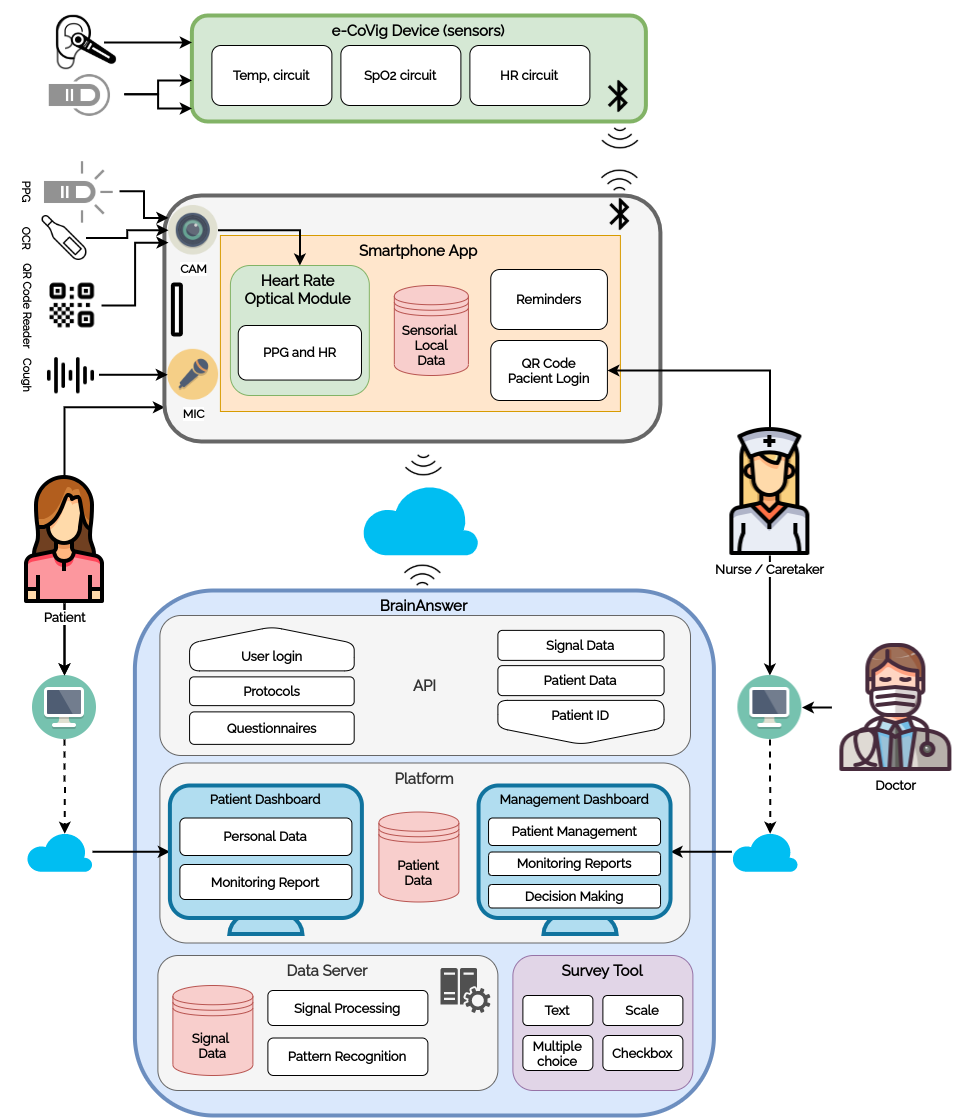
\includegraphics[width=0.60\linewidth]{images/ecovig.png}
    \caption[Diagram of e-Covig's system architecture.]{Overview of e-Covig's system architecture. Source: \cite{Raposo2021}.}
    \label{fig:ecovig-architecture}
\end{figure}


\subsection{Comparative Analysis}
% Baptiza cada trabalho com um nome teu, seguido da referencia.
\todo[inline]{Todo: Ver a questão de batizar os trabalhos.}
 \renewcommand{\arraystretch}{2}
  \begin{sidewaystable}[h]
      \centering
      \begin{tabular}{l|l|l|l|l|l|l}
        \textbf{References} & \makecell{\textbf{Measured} \textbf{Signals}} & \makecell{\textbf{Networking} \textbf{Protocols}}& \makecell{\textbf{Data} \textbf{Storage}} & \makecell{\textbf{e-Health} \textbf{Standards}} & \textbf{Features} & \textbf{Security Features} \\ \hline
          \cite{Fuhrer2006} & \xmark & \makecell{EPC/RFID,\\ Wi-Fi} & MySQL & None & \makecell{RTLS}& \makecell{Unspecified Storage \\Encryption} \\ \hdashline
          \cite{Adame2018} & \makecell{Temperature, \\Heart Rate,\\ Accelerometer} & \makecell{EPC/RFID,\\ Wi-Fi} & MySQL & None & \makecell{RTLS, \\ Fall Detection,\\ Vital signs\\ monitoring}& \makecell{AES-128, WPA-Personal} \\ \hdashline
          %\cite{Catarinucci2015} & \makecell{Temperature, \\ \acs{ECG}, Accelerometer,\\  Barometric Pressure,\\  Ambient Light} & \makecell{EPC/RFID, 6LowPAN,\\ CoAP} & MySQL & None & RTLS & ? \\
          \cite{Wu2020} & \makecell{Temperature, \\Heart Rate,\\ Accelerometer} & \makecell{BLE, Wi-Fi, \\ MQTT} & MySQL & None & \makecell{RTLS, \\ Fall Detection,\\ Vital signs\\ monitoring}& \makecell{AES-128} \\ \hdashline
          \cite{Doukas2012} & \makecell{Temperature, \\Heart Rate,\\ Accelerometer, \\$CO_2$ Sensor} & \makecell{\acs{BLE}, Wi-Fi, GPRS/3G \\ HTTP} & MySQL & None & \makecell{Fall Detection, \\ Vital signs \\ monitoring} & AES \\ \hdashline
          \cite{BrainAnswer} & \makecell{Temperature, \\Heart Rate,\\ Pulse Oximetry, \\ Respiration Rate } & \makecell{\acs{BLE} Wi-Fi} & Unknown & None & \makecell{Fall Detection,\\ Vital signs\\ monitoring, \\ Clinical decision\\  support } & Unknown \\ 
          %\cite{} & & & & & &  \\
        \end{tabular}
      \caption{Comparison between different pervasive healthcare applications.}
      \label{tab:comparsion-articles}
  \end{sidewaystable} 
 \renewcommand{\arraystretch}{1}

\clearpage
\subsection{Weaknesses of literature}
\todo[inline]{To-do: Review section later!}
\label{sec:weaknesses}

% Apenas identificas o problema da Interoperabilidade e Standards?
% Pensa tb nas questões de segurança e escalabilidade. 
% Pode não ser uma fraqueza/desafio comum a *todos* os trabalhos na literatura mas ser algo q nem sempre é bem resolvido.

%\subsubsection{Security and Privacy} 
% From the literature, we find that researchers ensure data security and privacy through 
%\subsubsection{Interoperability} 

Despite recent efforts, interoperability is still an issue of \acs{IoT} systems. Due to the lack of clear and concise industry standards and regulations, many manufacturers develop their own proprietary data formats and communication protocols, which hampers the integration of new resources since the systems are designed within closed ecosystems \cite{Rubi2019}. Moreover, the adoption of new systems can be often met with much objection from the clinical staff due to their mistrust of technology \cite{DursunErgezen2020}. 
To facilitate the deployment of new healthcare systems in hospitals, these need to be integrated easily in existing \acs{HIS}. \bigskip

Fortunately, there are several international initiatives to promote the use of \acs{IoT} in health in a standardized way, such as HIMSS (Healthcare Information and Management Systems Society) and the Personal Connected Health Alliance (PCHAlliance). PCHAlliance for example promotes the adoption of the Continua Design Guidelines (CDG), which facilitates the integration of personal health devices into health systems. These guidelines have been recognized by ITU (International Telecommunication Union) and the European Commission and are adopted by countries such as Denmark, Norway and the USA, among others \cite{PersonalConnectedHealthAlliance2017}. These guidelines describe a series of e-health standards like \acs{FHIR} which facilitate the exchange of information between systems, in order to ensure the implementations become truly interoperable.

% Within this project we aim to continue to expand the capabilities of the Continua Design Principles tofurther extend the software to collect the data that is being exchanged between sensors, gateways, and end services to make implementations truly interoperable.

% The PCHAlliance publishes and promotes the global adoption of standards and the implementation guidelines that unleash the massive amounts of medical-grade data that enables a more holistic perspective. Commercial ready software enables the rapid integration of these standards into your product. A conformity assessment program verifies that the standards have been properly and uniformly implemented.

\section{Statement of Contributions}

After studying the different approaches taken by researchers, and in context of the dissertation, we propose a novel fully modular \acs{IoT} infrastructure that uses the \acs{FHIR} standard in order to fully integrate the data in the existing \acs{HIS}, Glintt GlobalCare. Other researchers in the \acf{ISR} already developed wearable devices, designated ``biostickers'', using two different networking stacks — \acs{BLE} and \acs{EPC/RFID}. The system must ensure reliable and secure communications with the devices for each protocol, implementing the aforementioned security features in section \ref{sec:weaknesses}. From a hardware perspective, the system is composed of 3 different components, as seen Figure \ref{fig:wow-architecture}: the biostickers, that acquire the patient's physiological signals, the ``SmartBox'', which acts as a central node of the WBAN and aggregate the data and then communicates it to the gateway, and the ``Smart Gateway'', which serves as a fog server in order to mitigate latency and other computing issues and acts as the gateway to the \acs{HIS}. 

\begin{figure}[H]
    \centering
    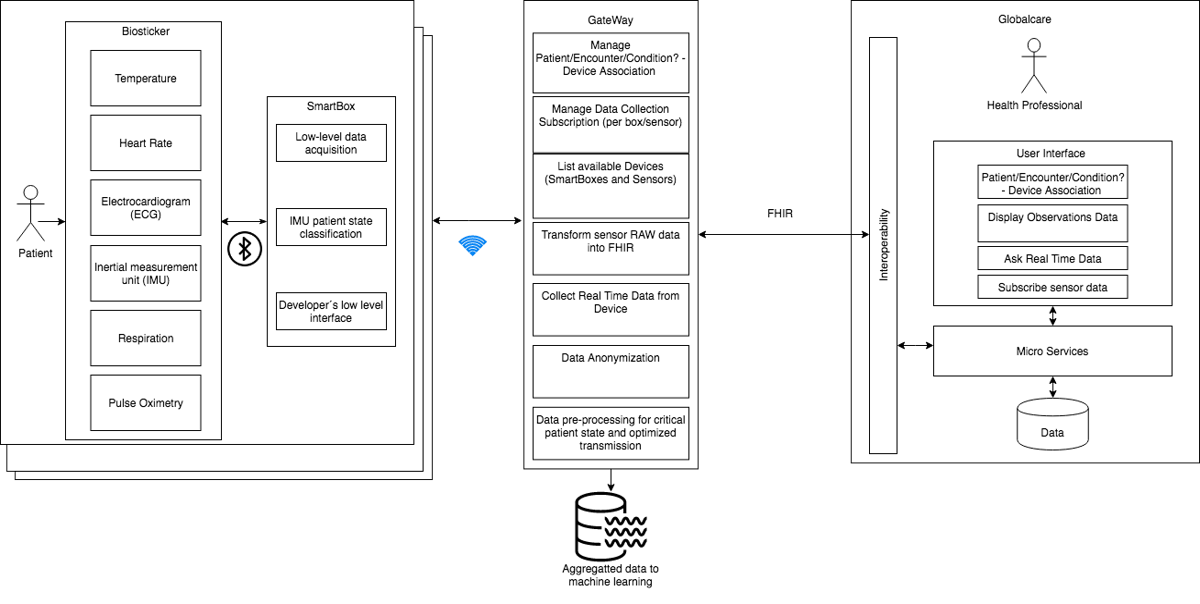
\includegraphics[width=\linewidth]{images/wow-architecture.png}
    \caption{System architecture of the \acs{WoW} project. The components highlighted in blue are discussed and implemented throughout this work.}
    \label{fig:wow-architecture}
\end{figure}

\todo[inline]{To-do: Replace image with a cleaner one. }

For the work developed throughout the dissertation, we have set the following goals: 

\begin{itemize}
    \item Develop and deploy SmartBoxes embedded in hospital beds for data acquisition from biostickers attached to patients’ skin:
    \begin{itemize}
        \item Hardware evaluation of 2 different \acs{IoT} kits (Raspberry Pi and Udoo Bolt).
        \item Viability study of a disruptive battery-less \acs{RFID} data acquisition compared to a \acs{BLE} acquisition.
        \item Implementation of reliable and secure \acs{RFID} data acquisition and general communication between the biosticker and the Smart Boxes.
        \item Selection of hardware components and assembly of SmartBox prototype;
    \end{itemize}
    \item Establishment of data integration pipelines using \acs{MQTT} and management of the multiple SmartBoxes in the Smart Gateway;
    \item Development of a \acs{FHIR} \acs{API} layer to integrate the proposed system in the GlobalCare \acs{HIS}.
    \item Evaluation of the performance of the proposed system through controlled lab tests and later deployment hospital trials within the WoW project.
    \item Evaluate the need for data analysis to extract relevant user profiles/anomalies for long-term biomonitoring data of multiple anonymous users.
\end{itemize}

\section{Summary}
In this chapter, we have discussed the importance of \acs{IoT} systems, how these are composed and how these can bring value to healthcare providers. After analyzing the different systems in the literature, their weaknesses and strengths, we have defined a set of criteria to guide the development of our own implementation.

\bigskip

In the next chapter, we begin with the hardware evaluation of the different \acs{IoT} kits and the implementation of secure communications between the biostickers and the SmartBoxes. 

% - Hardware evaluation for edge nodes which integrate electronic wireless patches that gather patient's physiological signals;
% - Integrating IoT system in an existing healthcare information system (Glintt GlobalCare software) through an FHIR API layer;
% - Evaluation of the performance of the proposed system through a testbed and a real healthcare scenario;

% In the context of the WoW project, a preliminary study will be performed, by analyzing 24 hours of data from 3 volunteers who are using a specific drug (i.e.! paracetamol) in order to illustrate the effect of the drug intake on various parameters, including temperature, emotions, heart rate, blood oxygen, and respiration.

% Se fizer sentido, na dissertação podes ter um capitulo de "Technological Background", que faz um overview às ferramentas de sotware e ao próprio hardware utilizado no projecto. (to be discussed later)

\bigskip